% Options for packages loaded elsewhere
% Options for packages loaded elsewhere
\PassOptionsToPackage{unicode}{hyperref}
\PassOptionsToPackage{hyphens}{url}
\PassOptionsToPackage{dvipsnames,svgnames,x11names}{xcolor}
%
\documentclass[
  letterpaper,
  DIV=11,
  numbers=noendperiod]{scrreprt}
\usepackage{xcolor}
\usepackage{amsmath,amssymb}
\setcounter{secnumdepth}{5}
\usepackage{iftex}
\ifPDFTeX
  \usepackage[T1]{fontenc}
  \usepackage[utf8]{inputenc}
  \usepackage{textcomp} % provide euro and other symbols
\else % if luatex or xetex
  \usepackage{unicode-math} % this also loads fontspec
  \defaultfontfeatures{Scale=MatchLowercase}
  \defaultfontfeatures[\rmfamily]{Ligatures=TeX,Scale=1}
\fi
\usepackage{lmodern}
\ifPDFTeX\else
  % xetex/luatex font selection
\fi
% Use upquote if available, for straight quotes in verbatim environments
\IfFileExists{upquote.sty}{\usepackage{upquote}}{}
\IfFileExists{microtype.sty}{% use microtype if available
  \usepackage[]{microtype}
  \UseMicrotypeSet[protrusion]{basicmath} % disable protrusion for tt fonts
}{}
\makeatletter
\@ifundefined{KOMAClassName}{% if non-KOMA class
  \IfFileExists{parskip.sty}{%
    \usepackage{parskip}
  }{% else
    \setlength{\parindent}{0pt}
    \setlength{\parskip}{6pt plus 2pt minus 1pt}}
}{% if KOMA class
  \KOMAoptions{parskip=half}}
\makeatother
% Make \paragraph and \subparagraph free-standing
\makeatletter
\ifx\paragraph\undefined\else
  \let\oldparagraph\paragraph
  \renewcommand{\paragraph}{
    \@ifstar
      \xxxParagraphStar
      \xxxParagraphNoStar
  }
  \newcommand{\xxxParagraphStar}[1]{\oldparagraph*{#1}\mbox{}}
  \newcommand{\xxxParagraphNoStar}[1]{\oldparagraph{#1}\mbox{}}
\fi
\ifx\subparagraph\undefined\else
  \let\oldsubparagraph\subparagraph
  \renewcommand{\subparagraph}{
    \@ifstar
      \xxxSubParagraphStar
      \xxxSubParagraphNoStar
  }
  \newcommand{\xxxSubParagraphStar}[1]{\oldsubparagraph*{#1}\mbox{}}
  \newcommand{\xxxSubParagraphNoStar}[1]{\oldsubparagraph{#1}\mbox{}}
\fi
\makeatother


\usepackage{longtable,booktabs,array}
\usepackage{calc} % for calculating minipage widths
% Correct order of tables after \paragraph or \subparagraph
\usepackage{etoolbox}
\makeatletter
\patchcmd\longtable{\par}{\if@noskipsec\mbox{}\fi\par}{}{}
\makeatother
% Allow footnotes in longtable head/foot
\IfFileExists{footnotehyper.sty}{\usepackage{footnotehyper}}{\usepackage{footnote}}
\makesavenoteenv{longtable}
\usepackage{graphicx}
\makeatletter
\newsavebox\pandoc@box
\newcommand*\pandocbounded[1]{% scales image to fit in text height/width
  \sbox\pandoc@box{#1}%
  \Gscale@div\@tempa{\textheight}{\dimexpr\ht\pandoc@box+\dp\pandoc@box\relax}%
  \Gscale@div\@tempb{\linewidth}{\wd\pandoc@box}%
  \ifdim\@tempb\p@<\@tempa\p@\let\@tempa\@tempb\fi% select the smaller of both
  \ifdim\@tempa\p@<\p@\scalebox{\@tempa}{\usebox\pandoc@box}%
  \else\usebox{\pandoc@box}%
  \fi%
}
% Set default figure placement to htbp
\def\fps@figure{htbp}
\makeatother





\setlength{\emergencystretch}{3em} % prevent overfull lines

\providecommand{\tightlist}{%
  \setlength{\itemsep}{0pt}\setlength{\parskip}{0pt}}



 


\KOMAoption{captions}{tableheading}
\makeatletter
\@ifpackageloaded{bookmark}{}{\usepackage{bookmark}}
\makeatother
\makeatletter
\@ifpackageloaded{caption}{}{\usepackage{caption}}
\AtBeginDocument{%
\ifdefined\contentsname
  \renewcommand*\contentsname{Table of contents}
\else
  \newcommand\contentsname{Table of contents}
\fi
\ifdefined\listfigurename
  \renewcommand*\listfigurename{List of Figures}
\else
  \newcommand\listfigurename{List of Figures}
\fi
\ifdefined\listtablename
  \renewcommand*\listtablename{List of Tables}
\else
  \newcommand\listtablename{List of Tables}
\fi
\ifdefined\figurename
  \renewcommand*\figurename{Figure}
\else
  \newcommand\figurename{Figure}
\fi
\ifdefined\tablename
  \renewcommand*\tablename{Table}
\else
  \newcommand\tablename{Table}
\fi
}
\@ifpackageloaded{float}{}{\usepackage{float}}
\floatstyle{ruled}
\@ifundefined{c@chapter}{\newfloat{codelisting}{h}{lop}}{\newfloat{codelisting}{h}{lop}[chapter]}
\floatname{codelisting}{Listing}
\newcommand*\listoflistings{\listof{codelisting}{List of Listings}}
\makeatother
\makeatletter
\makeatother
\makeatletter
\@ifpackageloaded{caption}{}{\usepackage{caption}}
\@ifpackageloaded{subcaption}{}{\usepackage{subcaption}}
\makeatother
\usepackage{bookmark}
\IfFileExists{xurl.sty}{\usepackage{xurl}}{} % add URL line breaks if available
\urlstyle{same}
\hypersetup{
  pdftitle={Muhammad Farrel Wibowo},
  pdfauthor={13523153 Muhammad Farrel Wibowo},
  colorlinks=true,
  linkcolor={blue},
  filecolor={Maroon},
  citecolor={Blue},
  urlcolor={Blue},
  pdfcreator={LaTeX via pandoc}}


\title{Muhammad Farrel Wibowo}
\usepackage{etoolbox}
\makeatletter
\providecommand{\subtitle}[1]{% add subtitle to \maketitle
  \apptocmd{\@title}{\par {\large #1 \par}}{}{}
}
\makeatother
\subtitle{Portfolio Asesmen II-2100 KIPP}
\author{13523153 Muhammad Farrel Wibowo}
\date{2027-07-10}
\begin{document}
\maketitle

\renewcommand*\contentsname{Table of contents}
{
\hypersetup{linkcolor=}
\setcounter{tocdepth}{2}
\tableofcontents
}

\bookmarksetup{startatroot}

\chapter*{Selamat Berjumpa}\label{selamat-berjumpa}
\addcontentsline{toc}{chapter}{Selamat Berjumpa}

\markboth{Selamat Berjumpa}{Selamat Berjumpa}

\begin{figure}[H]

{\centering \includegraphics[width=9.5\linewidth,height=\textheight,keepaspectratio]{../images/profile-pict.png}

}

\caption{About Me}

\end{figure}%

Muhammad Farrel Wibowo adalah mahasiswa Teknik Informatika Institut
Teknologi Bandung angkatan 2023. Lahir di Jakarta pada 18 Juni 2005,
kini menetap di Jatinangor untuk menjalani aktivitas perkuliahan,
sementara rumah keluarganya masih berada di Jakarta. Sejak kecil Farrel
sudah akrab dengan dunia teknologi---mulai dari smartphone, komputer,
hingga internet---yang menumbuhkan rasa ingin tahu tentang bagaimana
teknologi bekerja dan bagaimana ia dapat mengubah kehidupan manusia.

Sehari-hari, Farrel dikenal sebagai sosok yang disiplin, pekerja keras,
dan reflektif. Ia memiliki berbagai hobi seperti olahraga gym,
fotografi, otomotif, videografi, dan tenis. Namun di balik banyaknya
minat tersebut, benang merah yang mengikat semuanya adalah rasa ingin
belajar dan berkembang secara berkelanjutan.

\bookmarksetup{startatroot}

\chapter{UTS-1 All About Me}\label{uts-1-all-about-me}

\begin{figure}[H]

{\centering \includegraphics[width=9.5\linewidth,height=\textheight,keepaspectratio]{All_About_me/../images/profile-pict.png}

}

\caption{About Me}

\end{figure}%

Muhammad Farrel Wibowo adalah mahasiswa Teknik Informatika Institut
Teknologi Bandung angkatan 2023. Lahir di Jakarta pada 18 Juni 2005,
kini menetap di Jatinangor untuk menjalani aktivitas perkuliahan,
sementara rumah keluarganya masih berada di Jakarta. Sejak kecil Farrel
sudah akrab dengan dunia teknologi---mulai dari smartphone, komputer,
hingga internet---yang menumbuhkan rasa ingin tahu tentang bagaimana
teknologi bekerja dan bagaimana ia dapat mengubah kehidupan manusia.

Sehari-hari, Farrel dikenal sebagai sosok yang disiplin, pekerja keras,
dan reflektif. Ia memiliki berbagai hobi seperti olahraga gym,
fotografi, otomotif, videografi, dan tenis. Namun di balik banyaknya
minat tersebut, benang merah yang mengikat semuanya adalah rasa ingin
belajar dan berkembang secara berkelanjutan.

\section{\texorpdfstring{\textbf{Kisah yang Membentuk Diri Anda:
Mengenal Kekuatan Identitas
Naratif}}{Kisah yang Membentuk Diri Anda: Mengenal Kekuatan Identitas Naratif}}\label{kisah-yang-membentuk-diri-anda-mengenal-kekuatan-identitas-naratif}

Saya percaya bahwa setiap orang adalah pencerita alami yang menenun
kehidupannya menjadi sebuah kisah. Bagi saya, kisah itu dimulai dari
rasa ingin tahu yang sederhana terhadap teknologi, lalu berkembang
menjadi perjalanan penuh pembelajaran, perjuangan, dan pemaknaan diri.

Di masa SMA di MAN 4 Jakarta, saya mengambil jurusan Sains dan
Matematika dengan kurikulum Cambridge AS Level. Dari situlah saya mulai
memadukan logika dengan kreativitas. Saya bergabung di klub robotika dan
klub teknologi informasi, di mana saya belajar membangun robot serta
memprogramnya dengan Arduino IDE. Salah satu momen berharga adalah
ketika tim saya berhasil meraih medali perak pada ASEAN Innovative
Science \& Entrepreneur Fair (AISEF) berkat proyek Early Warning Flood
System berbasis Arduino, Wi-Fi, dan Blynk. Kemenangan itu bukan sekadar
prestasi, tetapi momen berkilau---saat saya menyadari bahwa teknologi
bukan hanya tentang kode dan alat, melainkan tentang solusi yang
menyentuh kehidupan manusia.

\subsection{\texorpdfstring{\textbf{1. Tiga Lapisan Diri Anda: Di Mana
Cerita Hidup Anda
Berada?}}{1. Tiga Lapisan Diri Anda: Di Mana Cerita Hidup Anda Berada?}}\label{tiga-lapisan-diri-anda-di-mana-cerita-hidup-anda-berada}

Mengikuti kerangka dari Dan P. McAdams, saya bisa memetakan perjalanan
diri saya sebagai berikut:

Level 1: Sifat Dasar. Saya cenderung disiplin, logis, dan berorientasi
pada hasil. Namun, di balik itu saya juga reflektif dan tenang---lebih
banyak mengamati sebelum bertindak.

Level 2: Kepedulian Pribadi. Nilai yang saya pegang adalah tanggung
jawab terhadap proses dan keberanian untuk menghadapi kegagalan. Saya
percaya bahwa setiap kesalahan adalah bentuk pembelajaran yang penting.

Level 3: Identitas Naratif. Inilah titik di mana seluruh lapisan diri
saya bertemu. Saya melihat diri saya sebagai seseorang yang terus
belajar dari masa lalu, memperjuangkan apa yang diinginkan, dan berusaha
berkontribusi lewat teknologi yang bermanfaat bagi orang lain.

Salah satu peristiwa yang paling membentuk identitas saya adalah ketika
saya gagal masuk perguruan tinggi melalui jalur SNBT. Kegagalan itu
sempat menimbulkan rasa kecewa, tetapi justru menjadi titik balik. Saya
belajar untuk bangkit, berjuang kembali melalui jalur Mandiri ITB, dan
akhirnya diterima di jurusan impian saya. Perjalanan itu mengajarkan
bahwa hasil besar tidak datang dari keberuntungan, melainkan dari
konsistensi dan keyakinan.

\subsection{\texorpdfstring{\textbf{2. Pola-Pola Kisah Kehidupan: Apa
yang Membuat Sebuah Cerita
Bermanfaat?}}{2. Pola-Pola Kisah Kehidupan: Apa yang Membuat Sebuah Cerita Bermanfaat?}}\label{pola-pola-kisah-kehidupan-apa-yang-membuat-sebuah-cerita-bermanfaat}

Cerita hidup saya mencerminkan pola penebusan (redemption)---dari
kegagalan menuju keberhasilan, dari keterbatasan menuju kesempatan baru.
Kegagalan masuk kampus favorit bukan akhir cerita, tetapi bab pembuka
dari narasi yang lebih bermakna. Kini, setelah menjadi mahasiswa, saya
juga mulai mengembangkan pola agensi dan koneksi, di mana peran saya
tidak lagi sebatas individu yang berjuang, tetapi bagian dari ekosistem
yang saling tumbuh bersama.

\begin{longtable}[]{@{}
  >{\raggedright\arraybackslash}p{(\linewidth - 2\tabcolsep) * \real{0.2097}}
  >{\raggedright\arraybackslash}p{(\linewidth - 2\tabcolsep) * \real{0.7903}}@{}}
\toprule\noalign{}
\endhead
\bottomrule\noalign{}
\endlastfoot
\textbf{Pola Naratif} & \textbf{Dampak Psikologis dan Pembelajaran
Pribadi} \\
\textbf{Penebusan} (Negatif → Positif) & Gagal di SNBT menjadi titik
balik untuk membangun ketekunan dan rasa percaya diri dalam meraih ITB
melalui jalur mandiri. \\
\textbf{Agensi} (Diri sebagai Aktor Efektif) & Mengembangkan kemampuan
kepemimpinan, pengambilan keputusan, dan inisiatif, seperti saat
memimpin proyek di TEC dan mengikuti hackathon. \\
\textbf{Koneksi} (Hubungan \& Rasa Memiliki) & Menemukan makna dalam
kerja sama tim dan kontribusi kolektif, misalnya saat menjadi staf HMIF
dan anggota ITB Jazz. \\
\textbf{Momen Berkilau} & Juara 3 \textbf{Hackathon} pertama saya di
perkuliahan menjadi simbol bagaimana kolaborasi, kecepatan berpikir, dan
disiplin teknis dapat membawa hasil. \\
\end{longtable}

\subsection{\texorpdfstring{\textbf{3. Seni Memberi Makna: Kekuatan
Super Anda dalam
Bernalar}}{3. Seni Memberi Makna: Kekuatan Super Anda dalam Bernalar}}\label{seni-memberi-makna-kekuatan-super-anda-dalam-bernalar}

Saya tidak pernah menganggap kesalahan sebagai musuh, melainkan guru.
Setiap kegagalan---baik dalam ujian, proyek, maupun
keputusan---membentuk cara berpikir saya yang lebih tenang dan
strategis. Selama berkuliah di ITB, saya menyadari bahwa menjadi
mahasiswa bukan hanya tentang menguasai algoritma atau pemrograman,
tetapi juga belajar bagaimana berpikir jernih di tengah tekanan dan
berinteraksi dengan berbagai karakter.

Momentum baru saya hadir ketika tim kami meraih Juara 3
Hackathon---lomba pertama saya selama kuliah. Selain validasi kerja tim,
kompetisi ini memberikan pembelajaran yang sangat praktis:

Framing masalah \& scoping MVP: menajamkan batas solusi agar berdampak
nyata dalam waktu terbatas.

Kolaborasi teknis di bawah tekanan waktu: branching Git yang rapi, code
review singkat namun tegas, dan keberanian membuat trade-off teknis.

Integrasi cepat \& reliability dasar: mengikat API, merapikan error
handling, serta memastikan demo berjalan stabil.

Storytelling produk: menyusun pitch yang jelas---dari problem statement,
insight pengguna, ke nilai guna---tanpa gimmick berlebihan.

Pengalaman ini menegaskan kembali bahwa agensi bukan semata kemampuan
teknis, melainkan keputusan-keputusan kecil yang konsisten: memilih
prioritas, menjaga ritme tim, dan bertanggung jawab atas kualitas hasil.

Kesadaran terbesar saya tetap sama: dunia ini tidak berputar di sekitar
diri saya sendiri. Setiap orang memiliki kisah, perjuangan, dan maknanya
masing-masing. Menyadari hal ini membuat saya lebih menghargai
keberagaman dan lebih rendah hati dalam proses belajar maupun
berorganisasi. Dari sinilah lahir keseimbangan antara ambisi dan empati.

\subsection{\texorpdfstring{\textbf{4. Mulai Menulis Ulang Kisah Anda:
Dua Langkah
Praktis}}{4. Mulai Menulis Ulang Kisah Anda: Dua Langkah Praktis}}\label{mulai-menulis-ulang-kisah-anda-dua-langkah-praktis}

Meskipun masa lalu tidak bisa diubah, saya menyadari bahwa cara saya
memaknainya bisa. Ada dua langkah yang terus saya latih agar tetap
tumbuh:

\subsubsection{Langkah 1: Eksternalisasi
Masalah}\label{langkah-1-eksternalisasi-masalah}

Saya belajar memisahkan identitas diri dari permasalahan yang saya
hadapi. Alih-alih berpikir ``saya gagal'', saya membingkai ulang menjadi
``saya sedang berhadapan dengan tantangan yang bisa saya atasi.''
Pergeseran cara berpikir ini mengubah rasa frustrasi menjadi ruang untuk
analisis dan perbaikan. Di dunia teknologi yang penuh trial-error,
kemampuan ini membuat saya lebih stabil dan berorientasi solusi.

\subsubsection{Langkah 2: Temukan Momen
Berkilau}\label{langkah-2-temukan-momen-berkilau}

Setiap kali saya merasa kehilangan arah, saya mencari kembali ``momen
berkilau'' yang pernah saya alami:

Ketika saya lolos ITB lewat jalur mandiri setelah gagal SNBT.

Saat dipercaya menjadi mentor di TEC untuk program pembelajaran data
science.

Ketika tim saya memenangkan Juara 3 Hackathon, yang memperkuat keyakinan
bahwa kerja keras kolektif dan visi yang jelas mampu mengubah tekanan
menjadi prestasi.

Momen-momen ini menjadi jangkar optimisme yang saya pegang, sekaligus
bukti bahwa perubahan naratif selalu mungkin.

\subsection{\texorpdfstring{\textbf{5. Kesimpulan: Kisah Saya Masih
Terus
Ditulis}}{5. Kesimpulan: Kisah Saya Masih Terus Ditulis}}\label{kesimpulan-kisah-saya-masih-terus-ditulis}

Perjalanan saya hingga saat ini bukanlah kisah yang sempurna, tetapi
kisah yang jujur. Saya belajar bahwa makna hidup tidak selalu datang
dari hasil yang besar, tetapi dari proses memahami diri sendiri dan
berkontribusi bagi sekitar.

Teknologi mungkin adalah bahasa yang saya pilih untuk mengekspresikan
diri, tetapi nilai yang ingin saya bawa jauh melampaui kode dan
algoritma---yakni ketekunan, rasa syukur, dan kesadaran bahwa setiap
keberhasilan adalah hasil dari perjuangan bersama.

Saya percaya bahwa kisah saya baru saja dimulai. Dan seperti dalam
setiap baris kode yang saya tulis, selalu ada ruang untuk perbaikan,
pembaruan, dan versi yang lebih baik dari diri saya sendiri.

\bookmarksetup{startatroot}

\chapter{UTS-2 My Songs for You}\label{uts-2-my-songs-for-you}

Dari Hati Performed by

Club Eighties

\url{https://youtu.be/USF8xr4QEa0?si=tu8tP-XTlD5Bz-b9}

\subsubsection{Makna dan Alasan Pemilihan
Lagu}\label{makna-dan-alasan-pemilihan-lagu}

Lagu ``Dari Hati'' dipilih karena memiliki makna yang sangat mendalam
tentang kejujuran, kesungguhan, dan ketulusan dalam mencintai seseorang.
Bagi saya, lagu ini menggambarkan bentuk cinta yang sederhana, jujur,
dan tanpa syarat---cinta yang tidak dibungkus oleh ambisi atau
kepemilikan, melainkan oleh keberanian untuk mengungkapkan perasaan yang
paling murni: ``Ku ingin jujur apa adanya, dari hati.''

Lagu ini menjadi inspirasi sekaligus refleksi untuk karya pribadi saya,
``My Songs for U'', yaitu sebuah lagu yang saya tulis dan ingin
nyanyikan pada hari pernikahan saya nanti. Lagu itu bukan sekadar
persembahan musik, tetapi bentuk nyata dari doa dan perasaan terdalam
terhadap pasangan saya kelak---bahwa cinta yang baik tidak perlu banyak
kata, cukup datang dari hati dan dijaga dengan sepenuh hati.

Seperti dalam lirik ``Dari Hati'', kejujuran menjadi fondasi yang saya
yakini harus hadir dalam setiap hubungan. Bagian ``Ku ingin kau menjadi
milikku, entah bagaimana caranya'' tidak dimaknai sebagai kepemilikan
egoistik, melainkan sebagai bentuk niat tulus untuk berbagi perjalanan
hidup bersama seseorang yang kita yakini sebagai belahan hati. Lirik
tersebut juga menandakan kerendahan hati di tengah ketidakpastian, bahwa
cinta tidak selalu bisa dikontrol, namun dapat dijaga dengan keikhlasan.

Bagi saya, lagu ini adalah narasi cinta dewasa---tentang seseorang yang
tidak lagi ingin menaklukkan, melainkan berjuang bersama; yang tidak
lagi bicara tentang ``aku dan kamu'', tetapi tentang ``kita''. Itulah
sebabnya saya ingin mengabadikan semangat yang sama melalui lagu ``My
Songs for U'', yang kelak akan saya nyanyikan pada hari pernikahan saya
sebagai simbol perjalanan hidup yang berpuncak pada makna: mencintai
dengan jujur, dari hati.

{[}Intro{]} Andai engkau tahu Bila menjadi aku, sejuta rasa di hati Lama
tlah kupendam Tapi akan kucoba mengatakannya

{[}Verse 1{]} Ku ingin kau menjadi milikku Entah bagaimana caranya
Lihatlah mataku untuk memintamu Ku ingin jalani bersamamu Coba dengan
sepenuh hati Ku ingin jujur apa adanya Dari hati

{[}Chorus 1{]} Kini engkau tahu aku menginginkanmu Tapi takkan
kupaksakan Dan kupastikan kau belahan hati Bila milikku oooo Ku ingin
kau menjadi milikku Entah bagaimana caranya Lihatlah mataku untuk
memintamu Aku ingin jalani bersamamu Coba dengan sepenuh hati Ku ingin
jujur apa adanya

{[}Bridge{]} Menarilah bersamaku Dengan bintang-bintang Sambutlah diriku
Untuk memelukmu

{[}Chorus 2{]} Ku ingin kau menjadi milikku Entah bagaimana caranya
Lihatlah mataku untuk memintamu Ku ingin jalani bersamamu Coba dengan
sepenuh hati Ku ingin jujur apa adanya Dari hati

{[}Outro{]} Dari hati

\bookmarksetup{startatroot}

\chapter{UTS-3 My Stories for You}\label{uts-3-my-stories-for-you}

\section{\texorpdfstring{\textbf{Sebuah Kisah: ``Belajar Menemukan Diri
di Tengah
Perjalanan''}}{Sebuah Kisah: ``Belajar Menemukan Diri di Tengah Perjalanan''}}\label{sebuah-kisah-belajar-menemukan-diri-di-tengah-perjalanan}

Hidup saya bukan rangkaian kemenangan, melainkan rangkaian proses
memahami arti kegagalan, kesabaran, dan keyakinan. Setiap langkah kecil
membawa pelajaran baru---dan kisah inilah yang ingin saya bagikan, bukan
karena sempurna, tetapi karena ia jujur dan membentuk siapa saya
sekarang.

\begin{center}\rule{0.5\linewidth}{0.5pt}\end{center}

\subsection{\texorpdfstring{\textbf{Awal
Perjalanan}}{Awal Perjalanan}}\label{awal-perjalanan}

Saya tumbuh sebagai anak yang selalu penasaran pada teknologi. Dari
komputer, internet, hingga robotik di SMA, semua itu membuat saya kagum
pada bagaimana sesuatu bisa ``hidup'' karena logika dan kode. Namun di
balik rasa ingin tahu itu, saya sering merasa belum cukup baik. Saya
takut gagal, takut tidak memenuhi ekspektasi.

Kegagalan pertama besar yang saya rasakan adalah saat tidak lolos
\textbf{SNBT}, ujian masuk perguruan tinggi yang selama ini saya
harapkan. Hari itu saya merasa dunia berhenti. Tetapi justru di titik
itu saya belajar makna \emph{penebusan}. Saya belajar bahwa hidup tidak
selalu harus berjalan lurus; kadang kita harus tersesat dulu untuk
benar-benar menemukan arah. Saya memutuskan mencoba jalur
\textbf{Mandiri ITB}, dan berhasil diterima di jurusan impian saya:
\textbf{Teknik Informatika Institut Teknologi Bandung}.

Sejak saat itu, saya memahami bahwa kegagalan bukan akhir cerita---ia
hanyalah tanda bahwa saya sedang ditulis ulang menjadi versi diri yang
lebih baik.

\begin{center}\rule{0.5\linewidth}{0.5pt}\end{center}

\subsection{\texorpdfstring{\textbf{Proses dan
Pembelajaran}}{Proses dan Pembelajaran}}\label{proses-dan-pembelajaran}

Perkuliahan di ITB bukan hanya tentang memahami algoritma atau teori,
tapi tentang membangun daya tahan mental. Di sinilah saya belajar
pentingnya keseimbangan antara ambisi dan empati.\\
Saya belajar menata waktu, menahan ego, menerima perbedaan cara
berpikir, dan memahami bahwa kesuksesan kolektif sering kali lebih
bermakna daripada kemenangan pribadi.

Puncak pengalaman itu datang ketika tim saya meraih \textbf{Juara 3
Hackathon pertama saya di bangku kuliah}.\\
Lomba itu bukan sekadar kompetisi, tapi ujian nyata tentang bagaimana
sebuah ide bisa diwujudkan di bawah tekanan waktu dan perbedaan
pendapat. Saya belajar banyak hal:\\
- Bahwa komunikasi adalah inti dari kolaborasi.\\
- Bahwa keputusan kecil, seperti siapa yang menulis kode terakhir atau
siapa yang mempresentasikan produk, bisa menentukan keberhasilan
bersama.\\
- Bahwa ketenangan dan rasa saling percaya lebih berharga daripada
kecepatan.

Sejak hari itu, saya menyadari bahwa kompetisi sejati bukan antara saya
dan orang lain---melainkan antara saya dan versi diri saya kemarin.

\begin{center}\rule{0.5\linewidth}{0.5pt}\end{center}

\subsection{\texorpdfstring{\textbf{Makna dan Inspirasi untuk Orang
Lain}}{Makna dan Inspirasi untuk Orang Lain}}\label{makna-dan-inspirasi-untuk-orang-lain}

Dari setiap perjalanan itu, saya ingin membagikan satu pesan
sederhana:\\
\textgreater{} ``Hidup tidak akan selalu berjalan sesuai rencana, tetapi
rencana Tuhan selalu berjalan sesuai kebutuhan kita.''

Kegagalan, kehilangan, bahkan ketidakpastian, semuanya adalah ruang
belajar untuk menemukan siapa diri kita sebenarnya.\\
Saya percaya bahwa setiap orang punya cerita yang bisa menyembuhkan
orang lain.\\
Dan jika kisah saya bisa membuat satu orang saja merasa lebih kuat untuk
bangkit, maka perjalanan ini sudah cukup berarti.

\begin{center}\rule{0.5\linewidth}{0.5pt}\end{center}

\subsection{\texorpdfstring{\textbf{Penutup: My Stories for
You}}{Penutup: My Stories for You}}\label{penutup-my-stories-for-you}

Lagu \emph{``Dari Hati''} yang saya pilih di tugas sebelumnya dan kisah
ini memiliki benang merah yang sama---\emph{kejujuran.}\\
Baik dalam cinta maupun dalam hidup, hanya kejujuran yang mampu menuntun
kita pada makna sejati.

Maka ``My Stories for You'' bukan hanya cerita tentang saya,\\
tetapi tentang keberanian untuk tetap percaya,\\
tentang proses menemukan arah di tengah ketidakpastian,\\
dan tentang bagaimana setiap kegagalan dapat berubah menjadi awal dari
sesuatu yang indah---\\
selama dijalani \textbf{dari hati.}

\bookmarksetup{startatroot}

\chapter{UTS-4 My SHAPE (Spiritual Gifts, Heart, Abilities, Personality,
Experiences)}\label{uts-4-my-shape-spiritual-gifts-heart-abilities-personality-experiences}

\begin{quote}
\textbf{Tujuan:} Merangkum rancangan diri (charter) agar saya melayani,
berkarya, dan memimpin secara paling selaras dengan karunia dan
pengalaman hidup saya. Dapat langsung ditempel ke halaman \textbf{UTS-4
--- My SHAPE} dan dipakai sebagai acuan aksi 90 hari.
\end{quote}

\section{\texorpdfstring{Sumber
\href{StrengthsProfile-Armein-Langi.pdf}{VIA
assessment}}{Sumber VIA assessment}}\label{sumber-via-assessment}

\section{0) Ringkasan 1 Halaman}\label{ringkasan-1-halaman}

\textbf{Peran Inti:} Profesor \& Elder --- perancang ekosistem
belajar-bernilai, pembimbing, dan pemimpin pelayanan komunitas.
\textbf{Misi:} Mengangkat kualitas hidup melalui \emph{smart
engineering} dan \emph{value-oriented education}, khususnya bagi
lansia/keluarga/komunitas (GRACE), serta pelayanan gerejawi yang
menumbuhkan kasih dan pengharapan. \textbf{Kekuatan Utama:} mengkonsep
sistem utuh, menulis \& mengajar, membangun jejaring, merancang
rubrik/alat evaluasi, menggerakkan proyek lintas-disiplin.
\textbf{Dampak yang Dituju:} karya, kurikulum, dan pelayanan yang
menumbuhkan karakter, keterampilan, serta kesejahteraan berkeadilan.

\textbf{Peta SHAPE (singkat):}

\begin{itemize}
\tightlist
\item
  \textbf{S --- Spiritual Gifts:} Teaching, Shepherding/Pastoring,
  Leadership, Wisdom/Discernment, Exhortation/Encouragement,
  Administration.
\item
  \textbf{H --- Heart (Minat \& Cinta Pelayanan):} pendidikan
  berorientasi nilai; kesejahteraan lansia \& keluarga (GRACE);
  pembinaan iman; menulis kisah/novel/lirik; rekayasa cerdas \& AI untuk
  kebaikan bersama; mentorship mahasiswa-dosen; penguatan jemaat.
\item
  \textbf{A --- Abilities (Kemampuan):} perancangan sistem (PSKVE/TISE),
  kurikulum \& rubrik, riset \& publikasi, menulis multi-format
  (Quarto/LaTeX), pemrograman (Python/R/Prolog/Modelica), komunikasi
  publik, memimpin kolaborasi.
\item
  \textbf{P --- Personality (Gaya Kepribadian Kerja):} strategis \&
  reflektif, berorientasi visi \& nilai, analitis-sistemik, kolaboratif,
  tenang dalam krisis, suka membangun standar \& alat.
\item
  \textbf{E --- Experiences (Pengalaman Kunci):} dosen \& peneliti
  lintas proyek (GRACE, Smart Engineering, pendidikan), Elder \&
  pengorganisasi jemaat, penulis kreatif, arsitek sistem pengetahuan
  (Obsidian/GitHub/Quarto), penggerak sarasehan \& penggalangan
  dukungan.
\end{itemize}

\begin{center}\rule{0.5\linewidth}{0.5pt}\end{center}

\section{1) S --- Spiritual Gifts (Karunia
Rohani)}\label{s-spiritual-gifts-karunia-rohani}

\begin{itemize}
\tightlist
\item
  \textbf{Teaching \& Wisdom/Discernment:} mengubah konsep kompleks
  menjadi peta belajar, rubrik, dan alat evaluasi yang memampukan.
\item
  \textbf{Shepherding/Pastoring \& Exhortation:} membimbing
  individu/kelompok dengan empati, meneguhkan, dan memberi arah.
\item
  \textbf{Leadership \& Administration:} merancang ekosistem
  (orang--proses--alat) dengan target berdampak dan terukur.
\end{itemize}

\textbf{Indikator Bukti:} silabus \& rubrik (II-2100/EL2007), naskah
pengajaran, bimbingan riset, modul/website kelas, program jemaat.

\begin{center}\rule{0.5\linewidth}{0.5pt}\end{center}

\section{2) H --- Heart (Minat, Nilai,
Kepedulian)}\label{h-heart-minat-nilai-kepedulian}

\begin{itemize}
\tightlist
\item
  Pendidikan yang \textbf{mencipta nilai} (CPMK↔rubrik↔artefak nyata).
\item
  \textbf{GRACE}: kualitas hidup lansia/keluarga melalui sistem dukung
  cerdas \& komunitas saling-melayani.
\item
  \textbf{Gereja \& Komunitas}: penguatan iman, kesalingan, dan
  pelayanan kasih.
\item
  \textbf{Kreativitas naratif}: kisah/novel/lirik sebagai sarana edukasi
  \& pengharapan.
\item
  \textbf{Rekayasa cerdas \& AI} untuk kemaslahatan.
\end{itemize}

\textbf{Masalah yang ingin dipecahkan:} kesenjangan antara
pengetahuan--karakter--aksi; pembelajaran kurang bermakna; layanan
komunitas belum terukur dampaknya.

\begin{center}\rule{0.5\linewidth}{0.5pt}\end{center}

\section{3) A --- Abilities (Kemampuan
Andal)}\label{a-abilities-kemampuan-andal}

\begin{itemize}
\tightlist
\item
  \textbf{Perancangan sistem} (PSKVE/TISE), \emph{value co‑creation},
  finansial rekayasa, desain instrumen penilaian.
\item
  \textbf{Kurikulum \& pedagogi}: CPMK↔rubrik↔tugas↔bukti; otomasi alur
  kerja (Python/Quarto/GitHub).
\item
  \textbf{Riset \& penulisan ilmiah}; \textbf{karya kreatif} (prosa,
  lirik, ceramah/khotbah).
\item
  \textbf{Teknis}: Python, R, Prolog (ontologi), Modelica, Quarto/LaTeX,
  Obsidian, GitHub, Graphviz.
\item
  \textbf{Komunikasi \& kepemimpinan}: orasi publik, fasilitasi
  sarasehan, negosiasi kolaborasi.
\end{itemize}

\begin{center}\rule{0.5\linewidth}{0.5pt}\end{center}

\section{4) P --- Personality (Gaya Kerja \&
Kolaborasi)}\label{p-personality-gaya-kerja-kolaborasi}

\begin{itemize}
\tightlist
\item
  \textbf{Strategis‑sistemik} (melihat gambaran besar, memetakan
  bagian-bagian).
\item
  \textbf{Reflektif \& nilai‑driven} (standar etis \& mutu).
\item
  \textbf{Kolaboratif} (membangun jejaring, memberi ruang tumbuh).
\item
  \textbf{Tenang‑tangguh} (fokus hasil jangka panjang).
\item
  \textbf{Pembelajar \& pembuat alat} (suka membuat template, rubrik,
  pipeline).
\end{itemize}

\begin{center}\rule{0.5\linewidth}{0.5pt}\end{center}

\section{5) E --- Experiences (Pengalaman
Pembentuk)}\label{e-experiences-pengalaman-pembentuk}

\begin{itemize}
\tightlist
\item
  \textbf{Akademik \& Riset:} merancang mata kuliah, SLR AI \&
  transformasi digital, proyek GRACE \& Smart Engineering.
\item
  \textbf{Pelayanan \& Organisasi:} Elder GKI, fasilitator sarasehan,
  penggalangan dukungan jemaat, pembinaan rohani.
\item
  \textbf{Kreasi Konten:} penulisan novel/khotbah/lirik; produksi materi
  ajar multi‑format.
\item
  \textbf{Infrastruktur Pengetahuan:} Obsidian--GitHub--Quarto, rubrik
  otomatis, bank soal.
\end{itemize}

\textbf{Pelajaran Inti:} integrasi iman--ilmu--nilai; sistem yang baik
melipatgandakan orang baik; narasi menggerakkan aksi.

\begin{center}\rule{0.5\linewidth}{0.5pt}\end{center}

\section{6) Piagam Diri (Self‑Charter)}\label{piagam-diri-selfcharter}

\textbf{Misi Hidup:} merancang dan menggerakkan ekosistem pembelajaran
\& pelayanan yang memerdekakan, bermakna, dan berkeadilan. \textbf{Nilai
Inti:} kasih, integritas, kebijaksanaan, keberanian, mutu, keberpihakan
pada yang lemah. \textbf{Peran Inti:} Perancang sistem
nilai‑pembelajaran; Pembimbing \& pengajar; Pemimpin pelayanan
komunitas. \textbf{Kompas Keputusan:} (1) Dampak pada manusia; (2)
Keselarasan nilai; (3) Keberlanjutan; (4) Kemampuan tim mengelola; (5)
Bukti terukur. \textbf{Janji Pelayanan:} hadir dengan empati, mendengar,
memberi arah praktis, membangun alat agar orang lain bertumbuh.
\textbf{Batasan:} menolak proyek yang mengabaikan martabat
manusia/etika; menjaga ritme kerja‑istirahat‑keluarga.

\begin{center}\rule{0.5\linewidth}{0.5pt}\end{center}

\section{7) Narasi 90 Detik (Elevator
Pitch)}\label{narasi-90-detik-elevator-pitch}

``Saya seorang profesor dan elder yang merancang ekosistem belajar dan
pelayanan berbasis nilai. Karunia saya mengajar, membimbing, dan
memimpin dengan pendekatan sistem: mengubah konsep besar menjadi peta,
rubrik, dan alat yang membuat orang bertumbuh. Hati saya pada pendidikan
bermakna, kesejahteraan lansia dan keluarga, serta penguatan jemaat.
Dengan pengalaman lintas riset, kurikulum, dan pelayanan, saya
menghubungkan ilmu, iman, dan aksi. Target saya sederhana: menghadirkan
karya dan komunitas yang saling menguatkan---di kelas, di gereja, dan di
masyarakat---agar lebih banyak orang hidup berkualitas, berpengharapan,
dan siap melayani.''

\begin{center}\rule{0.5\linewidth}{0.5pt}\end{center}

\section{8) Service‑Fit Map (Tempat Saya Paling
Berdampak)}\label{servicefit-map-tempat-saya-paling-berdampak}

\begin{itemize}
\tightlist
\item
  \textbf{Kampus:} perancangan kurikulum \& rubrik; mentorship riset;
  otomasi pipeline belajar; kuliah \& orasi.
\item
  \textbf{Jemaat:} pembinaan rohani \& khotbah; fasilitasi sarasehan;
  program lansia/keluarga (GRACE).
\item
  \textbf{Riset‑Inovasi:} desain platform nilai‑ciptakan (PSKVE);
  publikasi; konsorsium kolaborasi.
\item
  \textbf{Kreasi Naratif:} kisah/lirik sebagai media edukasi \&
  penguatan batin.
\end{itemize}

\begin{center}\rule{0.5\linewidth}{0.5pt}\end{center}

\section{9) Evidences (Artefak \&
Tautan)}\label{evidences-artefak-tautan}

\begin{quote}
Ganti tanda {[} {]} dengan tautan/berkas Anda.
\end{quote}

\begin{itemize}
\tightlist
\item[$\square$]
  Silabus \& rubrik II‑2100 / EL2007
\item[$\square$]
  Modul/website kelas \& bank soal
\item[$\square$]
  Khotbah/renungan \& materi sarasehan
\item[$\square$]
  Publikasi/SLR \& proposal riset (GRACE, dsb.)
\item[$\square$]
  Novel/lirik \& materi kreatif
\item[$\square$]
  Pipeline otomasi (Quarto/GitHub/Obsidian)
\end{itemize}

\begin{center}\rule{0.5\linewidth}{0.5pt}\end{center}

\section{10) Rencana Aksi 90 Hari
(SMART)}\label{rencana-aksi-90-hari-smart}

\begin{enumerate}
\def\labelenumi{\arabic{enumi}.}
\tightlist
\item
  \textbf{Rampungkan halaman UTS (KIPP/All‑About‑Me) end‑to‑end.}
  \emph{Outcome:} semua tugas berisi bukti + rubrik; \emph{Due:} T‑14
  hari.
\item
  \textbf{Mentor 3 tim mahasiswa menyusun artefak bernilai.}
  \emph{Outcome:} 3 proyek dengan metrik dampak; \emph{Due:} T‑45 hari.
\item
  \textbf{Pilot GRACE micro‑service di jemaat.} \emph{Outcome:} 1
  layanan kecil terukur (mis. pendampingan lansia); \emph{Due:} T‑90
  hari.
\item
  \textbf{Publikasi ringkas (working paper) integrasi
  iman--ilmu--nilai.} \emph{Outcome:} 1 naskah pra‑cetak; \emph{Due:}
  T‑75 hari.
\end{enumerate}

\begin{center}\rule{0.5\linewidth}{0.5pt}\end{center}

\section{11) SHAPE ↔ CPMK (Interpersonal \& Public
Communication)}\label{shape-cpmk-interpersonal-public-communication}

\begin{itemize}
\tightlist
\item
  \textbf{Self‑awareness \& refleksi (CPMK‑S):} dituangkan pada Piagam
  Diri \& Narasi 90 detik.
\item
  \textbf{Empati \& komunikasi etis (CPMK‑E):} Shepherding/Exhortation →
  khotbah, mentoring, review berempati.
\item
  \textbf{Storytelling \& presentasi (CPMK‑P):} Teaching + kreasi
  naratif → kuliah, cerita, lirik.
\item
  \textbf{Kolaborasi \& kepemimpinan (CPMK‑K):}
  Leadership/Administration → proyek riset/komunitas terukur.
\end{itemize}

\begin{center}\rule{0.5\linewidth}{0.5pt}\end{center}

\section{12) Self‑Assessment Rubrik UTS‑4 (isi
skormu)}\label{selfassessment-rubrik-uts4-isi-skormu}

\begin{longtable}[]{@{}
  >{\raggedright\arraybackslash}p{(\linewidth - 6\tabcolsep) * \real{0.3382}}
  >{\raggedright\arraybackslash}p{(\linewidth - 6\tabcolsep) * \real{0.4412}}
  >{\raggedleft\arraybackslash}p{(\linewidth - 6\tabcolsep) * \real{0.1471}}
  >{\raggedright\arraybackslash}p{(\linewidth - 6\tabcolsep) * \real{0.0735}}@{}}
\toprule\noalign{}
\begin{minipage}[b]{\linewidth}\raggedright
Kriteria
\end{minipage} & \begin{minipage}[b]{\linewidth}\raggedright
Deskripsi
\end{minipage} & \begin{minipage}[b]{\linewidth}\raggedleft
Skor (1--5)
\end{minipage} & \begin{minipage}[b]{\linewidth}\raggedright
Bukti
\end{minipage} \\
\midrule\noalign{}
\endhead
\bottomrule\noalign{}
\endlastfoot
Kelengkapan SHAPE & S‑H‑A‑P‑E jelas \& terisi & & \\
Koherensi Piagam Diri & misi‑nilai‑peran konsisten & & \\
Narasi 90 detik & ringkas, kuat, mengundang aksi & & \\
Evidence \& Aksi 90 hari & tautan bukti \& rencana SMART & & \\
\end{longtable}

\textbf{Total (maks 20):} {[} {]} \textbf{Tingkat:} ☐ A (≥85\%) ☐ B
(70--84\%) ☐ C (60--69\%) ☐ D (50--59\%) ☐ E (\textless50\%)

\begin{center}\rule{0.5\linewidth}{0.5pt}\end{center}

\section{13) Versi Ultra‑Ringkas (≤140
kata)}\label{versi-ultraringkas-140-kata}

``Saya profesor \& elder dengan karunia mengajar, membimbing, dan
memimpin secara sistemik. Hati saya pada pendidikan bernilai,
kesejahteraan lansia/keluarga (GRACE), dan penguatan jemaat. Kemampuan
saya merancang kurikulum, rubrik, dan alat otomasi belajar; menulis
ilmiah \& kreatif; serta menggerakkan kolaborasi. Pengalaman saya di
kampus, gereja, riset, dan kreasi konten mengajarkan integrasi
iman--ilmu--aksi. Misi saya menghadirkan ekosistem yang memerdekakan: di
kelas melalui pembelajaran bermakna; di jemaat melalui pelayanan kasih
yang terukur; dan di masyarakat melalui inovasi yang adil. Target 90
hari: menuntaskan artefak UTS, mementori 3 tim mahasiswa, memulai
layanan mikro GRACE, dan menerbitkan naskah ringkas.''

\section{Piagam Diri --- Armein Z. R.
Langi}\label{piagam-diri-armein-z.-r.-langi}

\textbf{Pernyataan Misi} Saya adalah insinyur-pendidik dan penulis yang
menyalakan sukacita belajar, menumbuhkan empati, dan merancang sistem
cerdas yang memuliakan Tuhan serta meningkatkan kualitas hidup keluarga,
kampus, dan komunitas. (Struktur mengikuti kerangka \emph{My
SHAPE}---Piagam Diri 1-halaman. )

\textbf{S --- Signature Strengths (inti kekuatan khas)} Humor,
Spiritualitas, Kreativitas, Suka Belajar, Keingintahuan, Pandangan
(wisdom/perspective), Bersyukur, Keadilan, Kecerdasan Sosial, Kejujuran,
Kepemimpinan. (Sumber: VIA Character Strengths Profile, 13 Okt 2025. )

\textbf{H --- Heart (nilai \& panggilan)} Empati sebagai kecerdasan
tertinggi; kebaikan lebih utama daripada sekadar pintar; pencarian ``The
True Reality''; sukacita hidup yang mengasihi; keluarga sebagai
ekosistem kasih. (Disimpulkan dari tulisan-tulisan Anda di blog:
\emph{Empati: Kecerdasan Tertinggi}; \emph{On Being Nice}; \emph{The
Truth, The True Reality}; tagline blog; catatan keluarga.
(\href{https://ii-2100.github.io/all-about-me/}{Armein Z. R. Langi in
the City of Eden}))

\textbf{A --- Aptitudes \& Acquired Skills (bakat \& keterampilan
kunci)} Perancangan \& penelitian sistem/komputasi (speech compression,
FPGA), rekayasa \& kurikulum, kepemimpinan akademik, penulisan \&
penceritaan, fasilitasi pembelajaran, sistem \& organisasi. (Contoh
teknis: riset speech compression \& desain kontrol prosesor pada awal
karier.
(\href{https://ii-2100.github.io/all-about-me/My_Song_for_You/index.html}{Armein
Z. R. Langi in the City of Eden}))

\textbf{P --- Personality (gaya kerja yang menonjol)}
Reflektif-analitis, empatik-inklusif, visioner, pembelajar antusias,
kolaboratif; berpihak pada keadilan \& integritas. (Disintesis dari pola
kekuatan VIA dan tema tulisan Anda. )

\textbf{E --- Experiences (jejak pembentuk identitas)}

\begin{itemize}
\tightlist
\item
  \textbf{Ketangguhan pribadi} --- ``The Child Who Learned to Walk at
  the Disneyland'': ketekunan, berjalan dalam dingin, terus melangkah
  menuju tujuan.
  (\href{https://ii-2100.github.io/all-about-me/My_Stories_for_You/index.html}{Armein
  Z. R. Langi in the City of Eden})
\item
  \textbf{Lompatan kompetensi awal} --- perjalanan riset: software
  speech compression jadi dalam 3 bulan; desain chip kontrol di Xilinx
  FPGA; menulis paper.
  (\href{https://ii-2100.github.io/all-about-me/My_Song_for_You/index.html}{Armein
  Z. R. Langi in the City of Eden})
\item
  \textbf{Keluarga \& komunitas} --- keluarga besar sebagai sumber
  nilai, pelayanan, dan sukacita.
  (\href{https://ii-2100.github.io/all-about-me/My_Shapes/index.html}{Armein
  Z. R. Langi in the City of Eden})
\item
  \textbf{Standar keunggulan} --- sensibilitas benchmarking sains \&
  pendidikan (refleksi tentang Caltech).
  (\href{https://ii-2100.github.io/all-about-me/My_Personal_Reviews/index.html}{Armein
  Z. R. Langi in the City of Eden})
\end{itemize}

\textbf{Janji Praktis (Operating Principles)}

\begin{enumerate}
\def\labelenumi{\arabic{enumi}.}
\tightlist
\item
  \emph{People first with empathy} • 2) \emph{Truth-seeking with
  humility} • 3) \emph{Design for value \& justice} • 4) \emph{Teach
  what I practice, practice what I teach} • 5) \emph{Joyful learning,
  faithful living}. (Kerangka dan cara merangkum diadaptasi dari
  \emph{My SHAPE Toolkit}. )
\end{enumerate}

\begin{center}\rule{0.5\linewidth}{0.5pt}\end{center}

\section{Narasi Diri (versi 90 detik)}\label{narasi-diri-versi-90-detik}

Saya Armein---insinyur, pendidik, dan penulis---yang percaya bahwa
pengetahuan hanya bermakna bila melahirkan kasih dan keadilan. Kekuatan
saya adalah \textbf{spiritualitas yang membumi, kreativitas rekayasa,
dan kegembiraan belajar tanpa henti}, yang saya pakai untuk menyalakan
semangat orang lain.

Perjalanan saya ditempa oleh pengalaman yang mengajarkan
\textbf{ketekunan}---mulai dari ``berjalan dalam dingin'' hingga tuntas
menyelesaikan riset komputasi dan merancang sistem sejak awal karier.
Keluarga dan komunitas menjadi ekosistem kasih tempat saya belajar bahwa
\textbf{kebaikan lebih tinggi nilainya daripada sekadar pintar} dan
\textbf{empati adalah kecerdasan tertinggi}.
(\href{https://ii-2100.github.io/all-about-me/My_Stories_for_You/index.html}{Armein
Z. R. Langi in the City of Eden})

Ke depan, saya ingin terus \textbf{mendesain lingkungan belajar dan
sistem cerdas} yang memuliakan Tuhan dan membawa berkat
nyata---membentuk insan pembelajar yang jujur, adil, dan penuh
syukur---seraya menjaga sukacita: \emph{joy of loving and exciting
life}.
(\href{https://ii-2100.github.io/all-about-me/My_Stories_for_You/index.html}{Armein
Z. R. Langi in the City of Eden})

\begin{center}\rule{0.5\linewidth}{0.5pt}\end{center}

\section{Narasi Diri (versi panjang, 3--5
paragraf)}\label{narasi-diri-versi-panjang-35-paragraf}

\textbf{Kini.} Saya mengabdikan diri sebagai insinyur-pendidik yang
merancang pengalaman belajar dan sistem cerdas agar manusia bertumbuh
utuh: cakap teknis, peka nurani, dan gembira belajar. Kekuatan
saya---spiritualitas, kreativitas, suka belajar, keingintahuan,
perspektif, keadilan, dan kepemimpinan---mengarahkan cara saya memimpin,
mengajar, dan menulis.

\textbf{Dulu---titik balik.} Saya belajar bahwa langkah kecil yang
konsisten mengalahkan rintangan besar: berjalan sendirian dalam
dingin---secara harfiah dan metaforis---membentuk ketahanan batin. Di
laboratorium, saya menuntaskan perangkat lunak \textbf{speech
compression} dalam waktu singkat dan merancang \textbf{control unit}
berbasis FPGA, lalu menulis paper pertama---momen yang mengajarkan
disiplin, standar mutu, dan keberanian intelektual.
(\href{https://ii-2100.github.io/all-about-me/My_Stories_for_You/index.html}{Armein
Z. R. Langi in the City of Eden})

\textbf{Nilai yang saya pegang.} Saya memilih \textbf{kebaikan} di atas
sekadar \textbf{kepintaran}, menempatkan \textbf{empati} sebagai
kecerdasan tertinggi, dan mengejar \textbf{kebenaran sebagai realitas
yang sesungguhnya}. Keluarga besar meneguhkan panggilan itu---rumah
sebagai laboratorium kasih dan keadilan.
(\href{https://azrl.wordpress.com/2010/01/09/on-being-nice/?utm_source=chatgpt.com}{Armein
Z. R. Langi in the City of Eden})

\textbf{Ke depan.} Dengan kerangka \textbf{My SHAPE}, saya terus
menyelaraskan kekuatan, nilai, keterampilan, gaya kerja, dan pengalaman
untuk merancang program, riset, dan karya tulis yang berdampak---agar
teknologi menjadi pelayan kemanusiaan, dan setiap ruang belajar menjadi
\emph{City of Eden}: tempat sukacita, kasih, dan keunggulan bertemu.

\bookmarksetup{startatroot}

\chapter{UTS-5 My Personal Reviews}\label{uts-5-my-personal-reviews}

Berikut cara saya melakukan review: mengguan chatGPT, saya mengattach
\href{skor_uts.pdf}{file promt ChatGPT}, disertai perintah :``self
assess uts-1 sanpai uts-5 dari URL
`https://ii-2100.github.io/all-about-me/'\,''

ChatGPT melakukan self-assessment UTS-1 s.d. UTS-5 langsung dari laman
yang Anda berikan dan menilai memakai rubrik tugas UTS (skala 1--5 per
kriteria). Rekap skor siap diunduh sebagai CSV:
\href{sandbox:/mnt/data/UTS_self_assessment.csv}{Download CSV
ringkasan}.

\bookmarksetup{startatroot}

\chapter{Hasil Self-Assessment UTS (URL:
ii-2100.github.io/all-about-me)}\label{hasil-self-assessment-uts-url-ii-2100.github.ioall-about-me}

\section{Identifikasi}\label{identifikasi}

\begin{itemize}
\tightlist
\item
  Nama \& NIM penulis: \textbf{Armein Z. R. Langi -- 131902360} (tertera
  di halaman depan portofolio).
  (\href{https://ii-2100.github.io/all-about-me/}{II 2100})
\item
  Penilai: \textbf{Self-assessment (Armein Z. R. Langi)}
\item
  Catatan cakupan: halaman beranda memuat ``About Me''; navigasi ke ``My
  Songs for You'', ``My Stories for You'', ``My Shapes'', dan ``My
  Personal Reviews'' tersedia.
  (\href{https://ii-2100.github.io/all-about-me/}{II 2100})
\end{itemize}

\section{Tinjauan Umum}\label{tinjauan-umum}

\begin{itemize}
\tightlist
\item
  \textbf{UTS-1 (All About Me)} hadir di beranda (``Selamat Berjumpa /
  About Me''). Isi memperkenalkan identitas dan latar personal secara
  padat. (\href{https://ii-2100.github.io/all-about-me/}{II 2100})
\item
  \textbf{UTS-2 (My Songs for You)} memuat judul karya dan tautan audio,
  namun lirik/isi tidak ditampilkan di halaman (file audio tidak bisa
  saya akses dari sini), sehingga penilaian konten terbatas pada
  kelengkapan presentasi.
  (\href{https://ii-2100.github.io/all-about-me/My_Song_for_You/index.html}{II
  2100})
\item
  \textbf{UTS-3 (My Stories for You)} berisi tautan ke beberapa cerita;
  konten naratif kuat, terutama pada kisah keluarga ``Gaun Pengantin
  Gladys'' serta kisah inspiratif lainnya.
  (\href{https://ii-2100.github.io/all-about-me/My_Stories_for_You/index.html}{II
  2100})
\item
  \textbf{UTS-4 (My SHAPE)} saat ini halaman kosong/tanpa isi, hanya
  navigasi.
  (\href{https://ii-2100.github.io/all-about-me/My_Shapes/index.html}{II
  2100})
\item
  \textbf{UTS-5 (My Personal Reviews)} berisi metode/tautan panduan
  review, namun belum ada contoh \textbf{review personal} yang lengkap
  terhadap sebuah pesan/teks.
  (\href{https://ii-2100.github.io/all-about-me/My_Personal_Reviews/index.html}{II
  2100})
\end{itemize}

\begin{center}\rule{0.5\linewidth}{0.5pt}\end{center}

\section{Tinjauan Spesifik + Skor
(1--5)}\label{tinjauan-spesifik-skor-15}

\subsection{UTS-1 --- All About Me (di
beranda)}\label{uts-1-all-about-me-di-beranda}

\textbf{Skor per kriteria:} Orisinalitas \textbf{3}, Keterlibatan
\textbf{3}, Humor \textbf{1}, Wawasan/Insight \textbf{3} → \textbf{Total
10/20 (50\%)}. \textbf{Alasan singkat:} Perkenalan diri faktual dan
jelas, namun gaya masih informatif ketimbang naratif (minim humor dan
moment ``hook''). (\href{https://ii-2100.github.io/all-about-me/}{II
2100}) \textbf{Saran perbaikan:} Buka dengan anekdot pribadi (1--2
paragraf) yang ``mengikat'' (mis. titik balik karier/keluarga),
tambahkan satu momen humor ringan, lalu tutup dengan refleksi singkat
tentang nilai/visi diri agar aspek insight naik.

\subsection{UTS-2 --- My Songs for You}\label{uts-2-my-songs-for-you-1}

\textbf{Skor per kriteria:} Orisinalitas \textbf{2}, Keterlibatan
\textbf{2}, Humor \textbf{1}, Inspirasi \textbf{2} → \textbf{Total 7/20
(35\%)}. \textbf{Alasan singkat:} Halaman menampilkan judul lagu ``River
in my Mind'', ``Heaven on Earth'', namun tanpa lirik/cerita di balik
lagu sehingga sulit menilai aspek pesan, humor, dan inspirasi.
(\href{https://ii-2100.github.io/all-about-me/My_Song_for_You/index.html}{II
2100}) \textbf{Saran perbaikan:} Tambahkan lirik lengkap, 1 paragraf
cerita proses kreatif, dan 2--3 kalimat ``pesan untukmu'' agar inspirasi
terbaca; sertakan player/tautan yang dapat diputar langsung + fallback
transkrip.

\subsection{UTS-3 --- My Stories for
You}\label{uts-3-my-stories-for-you-1}

\textbf{Skor per kriteria:} Orisinalitas \textbf{5}, Keterlibatan
\textbf{5}, Pengembangan Narasi \textbf{4}, Inspirasi \textbf{5} →
\textbf{Total 19/20 (95\%)}. \textbf{Alasan singkat:} Cerita ``Gaun
Pengantin Gladys'' dkk sangat personal, emosional, dan inspiratif; ritme
bertutur hidup serta detail situasional kuat (konten ramu unsur
penebusan/keluarga/iman).
(\href{https://ii-2100.github.io/all-about-me/My_Stories_for_You/index.html}{II
2100}) \textbf{Saran perbaikan:} Tambah ``lead'' 2--3 kalimat yang
merangkum pesan kunci tiap cerita; akhiri dengan ajakan/refleksi 1--2
kalimat agar resonansi ke pembaca makin jelas.

\subsection{UTS-4 --- My SHAPE}\label{uts-4-my-shape}

\textbf{Skor per kriteria:} Orisinalitas \textbf{1}, Keterlibatan
\textbf{1}, Pengembangan \textbf{1}, Inspirasi \textbf{1} →
\textbf{Total 4/20 (20\%)}. \textbf{Alasan singkat:} Konten belum
tersedia.
(\href{https://ii-2100.github.io/all-about-me/My_Shapes/index.html}{II
2100}) \textbf{Saran perbaikan (prioritas):}

\begin{enumerate}
\def\labelenumi{\arabic{enumi}.}
\tightlist
\item
  Tampilkan rekap SHAPE (Spiritual gifts, Heart, Abilities, Personality,
  Experiences) dalam 1 tabel ringkas + 3--5 butir bukti;
\item
  Narasikan 2 pengalaman kunci (±150 kata/each) yang menunjukkan
  ``signature strengths'';
\item
  Tutup dengan 3 rencana aksi konkret (who/what/when).
\end{enumerate}

\subsection{UTS-5 --- My Personal
Reviews}\label{uts-5-my-personal-reviews-1}

\textbf{Skor per kriteria:} Pemahaman Konsep \textbf{2}, Analisis Kritis
\textbf{1}, Argumentasi (Logos) \textbf{1}, Etos \& Empati \textbf{2},
Rekomendasi \textbf{1} → \textbf{Total 7/25 (28\%)}. \textbf{Alasan
singkat:} Halaman berisi metode cara menilai, tetapi \textbf{belum ada}
contoh \textbf{review personal} yang lengkap terhadap sebuah pesan/teks
sehingga aspek analisis-argumentasi tak terbaca.
(\href{https://ii-2100.github.io/all-about-me/My_Personal_Reviews/index.html}{II
2100}) \textbf{Saran perbaikan:} Pilih 1 karya personal (mis.
UTS-1/2/3), tulis review 400--600 kata: ringkas pesan, nilai dengan
rubrik, berikan 2--3 bukti kutipan, evaluasi etos/empati, lalu tutup
dengan rekomendasi perbaikan spesifik.

\begin{center}\rule{0.5\linewidth}{0.5pt}\end{center}

\section{Rekap Skor (ringkas)}\label{rekap-skor-ringkas}

\begin{itemize}
\tightlist
\item
  \textbf{UTS-1:} 10/20 → \textbf{50\%}
\item
  \textbf{UTS-2:} 7/20 → \textbf{35\%}
\item
  \textbf{UTS-3:} 19/20 → \textbf{95\%}
\item
  \textbf{UTS-4:} 4/20 → \textbf{20\%}
\item
  \textbf{UTS-5:} 7/25 → \textbf{28\%}
\end{itemize}

CSV lengkap sudah saya siapkan untuk dokumentasi dan olah lanjut:
\href{sandbox:/mnt/data/UTS_self_assessment.csv}{Download CSV
ringkasan}.

\section{Langkah Perbaikan Cepat (prioritas 1
minggu)}\label{langkah-perbaikan-cepat-prioritas-1-minggu}

\begin{enumerate}
\def\labelenumi{\arabic{enumi}.}
\tightlist
\item
  \textbf{Lengkapi UTS-4 (My SHAPE)} sesuai saran di atas;
\item
  \textbf{Tambahkan lirik + sinopsis} untuk tiap lagu di UTS-2 agar bisa
  dinilai isi/inspirasinya;
\item
  \textbf{Tulis 1 review personal penuh} (UTS-5) memakai rubrik (pilih
  salah satu karya Anda sendiri sebagai objek);
\item
  Revisi UTS-1 dengan pembuka anekdot + refleksi nilai diri.
\end{enumerate}

Jika Anda mau, saya bisa bantu merapikan UTS-4 (tabel SHAPE + narasi)
dan membuat kerangka cepat untuk \textbf{review} di UTS-5 dari salah
satu karya Anda.

\bookmarksetup{startatroot}

\chapter{UAS-1 My Concepts}\label{uas-1-my-concepts}

Mau hidup epik ? \href{lifestory.pdf}{Write your Life Story}

Apa itu berkonsep?

\url{https://youtu.be/QVfUlVBO80U?si=yM6q_rwV9rcDBbu7}

\bookmarksetup{startatroot}

\chapter{UAS-3 My Opinions}\label{uas-3-my-opinions}

SApa itu beropini? \href{BM\%20Opini.mp4}{Opini Berpengaruh}

Bagiamana menjaadi menarik? \href{./Interesting.mp4}{Menjadi Menarik}

\bookmarksetup{startatroot}

\chapter{UAS-3 My Innovations}\label{uas-3-my-innovations}

\bookmarksetup{startatroot}

\chapter{UAS-4 My Knowledge}\label{uas-4-my-knowledge}

Cara saya mengkomunikasikan sebuah pengatahuan sebagai petunjuk bagi
orang lain 1) saya tulis
\href{Rekomendasi\%20Presentasi\%20Efektif(Contoh\%20Makalah).pdf}{makalah
sebagai bahan utama} 2) lalu saya buat
\href{Contoh\%20Transkrip\%20Presentasi.pdf}{transkrip ucapan lisan} 3)
kemudian saya kembangkan
\href{Rekomendasi\%20Presentasi\%20(Contoh\%20Slides).pdf}{slide
pendukung trnsskrip} 4) lalu saya memproduksivideo audio visual
\url{https://youtu.be/ZbghfMvnPZc} \url{https://youtu.be/ZbghfMvnPZc}

\bookmarksetup{startatroot}

\chapter{UAS-5 My Professional
Reviews}\label{uas-5-my-professional-reviews}

Untuk melAkukan review, seperti pada
\href{../My_Personal_Reviews/Doc.5.Mengevaluasi-Esai-Berdasarkan-Rubrik.pdf}{pendekatan
AI}, kita membutuhkan rubrik

\bookmarksetup{startatroot}

\chapter{Summary}\label{summary}

In summary, this book has no content whatsoever.

\bookmarksetup{startatroot}

\chapter*{References}\label{references}
\addcontentsline{toc}{chapter}{References}

\markboth{References}{References}

\phantomsection\label{refs}




\end{document}
